\subsection{SP8: análisis exploratorio de escala}
\label{sec:resultados-sp8}

\subsubsection{Pregunta y alcance implementado}

SP8 explora cómo cambian salidas agregadas del modelo cuando la flota crece desde $N=5$ hasta $N=50\,000$. Los tamaños mayores se representan mediante variables mesoscópicas por zona y no mediante trayectorias individuales. La campaña histórica combina métricas de calidad con reglas analíticas de coste,
\[
 m(N)=\bigl(r_{\rm comp},r_{\rm wrench},\widehat t_{\rm cpu},
 \widehat M_{\rm mem},n_{\rm msg},r_{\rm lim}\bigr).
\]
Los símbolos con sombrero indican estimaciones o valores declarados por el evaluador. No son mediciones de wall-clock o RSS.

\begin{figure}[htbp]
\centering
\resizebox{0.94\textwidth}{!}{%
\begin{tikzpicture}[
  font=\sffamily\small,
  regime/.style={draw=VIUDark!70,fill=VIUWhite,rounded corners=3pt,align=center,minimum height=1.25cm,text width=3.45cm,inner sep=5pt},
  active/.style={draw=VIUOrange!90!black,fill=VIUOrange!12,rounded corners=3pt,align=center,minimum height=1.25cm,text width=3.45cm,inner sep=5pt},
  flow/.style={-{Latex[length=2.6mm]},line width=0.95pt,draw=VIUDark!75}
]
\node[regime] (small) at (0,0) {Escala peque\~na\\$N=5$--$50$\\referencias globales};
\node[regime] (medium) at (4.8,0) {Escala intermedia\\$N=10^2$--$10^3$\\m\'etodos distribuidos};
\node[active] (large) at (9.6,0) {Escala mesosc\'opica\\$N=10^4$--$5\times10^4$\\aproximaciones agregadas};
\draw[flow] (small) -- node[above,font=\scriptsize] {tiempo y memoria} (medium);
\draw[flow] (medium) -- node[above,font=\scriptsize] {mensajes y cierres} (large);
\draw[VIUDark!55,line width=0.8pt] (-1.8,-1.45) -- (11.4,-1.45);
\foreach \x/\lab in {-1.5/5,0.0/50,3.0/$10^2$,5.0/$10^3$,8.1/$10^4$,10.9/$5\cdot10^4$}{
  \draw[VIUDark!55] (\x,-1.55)--(\x,-1.35);
  \node[below,font=\scriptsize] at (\x,-1.58) {\lab};
}
\node[below=7mm,font=\scriptsize] at (4.8,-1.45) {tama\~no de flota $N$};
\end{tikzpicture}}
\caption[Reg\'imenes de escala evaluados en SP8]{Reg\'imenes de escala de SP8. Las flotas mayores se estudian mediante un modelo mesosc\'opico que no equivale a una prueba en una instalaci\'on real.}
\viuownsource
\label{fig:sp8-scale-regimes}
\end{figure}


\subsubsection{Métodos y diseño histórico}

\begin{table}[H]
\centering
\scriptsize
\begin{tabularx}{\textwidth}{@{}p{0.31\textwidth}p{0.18\textwidth}X@{}}
\toprule
Método & Alcance & Función en SP8 \\
\midrule
Oráculo de coalición y MPC temporal & Proxies centralizados & Referencias expandidas con coste declarado. \\
Húngaro expandido & Centralizado adaptado & Asignación clásica dentro del modelo agregado. \\
\emph{Greedy}, subasta y CBBA local & Proxies distribuidos & Referencias de baja coordinación. \\
Aproximación de campo medio & Descentralizado & Opera sobre densidades agregadas. \\
Primal-dual espacial & Proxy descentralizado & Distribuye precios por zona. \\
Flujo tensorial de cuórum & Proxy descentralizado & Cierra cuórums mediante campos agregados. \\
Mercado \emph{wrench} jerárquico & Jerárquico & Combina resúmenes de zona y pujas locales. \\
\bottomrule
\end{tabularx}
\caption{Métodos y alcance de implementación en la campaña histórica SP8.}
\label{tab:sp8-methods}
\end{table}

El diseño programa veinte tamaños y cien semillas por tamaño para diez métodos, lo que produce $20\,000$ filas de protocolo. Una fila programada no equivale necesariamente a una ejecución observada: las ramas que declaran límite, omiten cálculo o asignan una salida nula deben distinguirse de timeout, error y solución. Además, \texttt{route\_mitigation} y las reglas de completitud dependen de la identidad del
método; una diferencia de calidad mezcla por tanto política y evaluador. Las fórmulas de
memoria y mitigación también dependen del método. Los contrastes H8.2--H8.3 no se
interpretan como efectos causales entre algoritmos, y estas decisiones impiden una
comparación confirmatoria de coste computacional.

\subsubsection{Resultados descriptivos}

\begin{figure}[H]
\centering
\begin{minipage}[t]{0.49\textwidth}
\centering
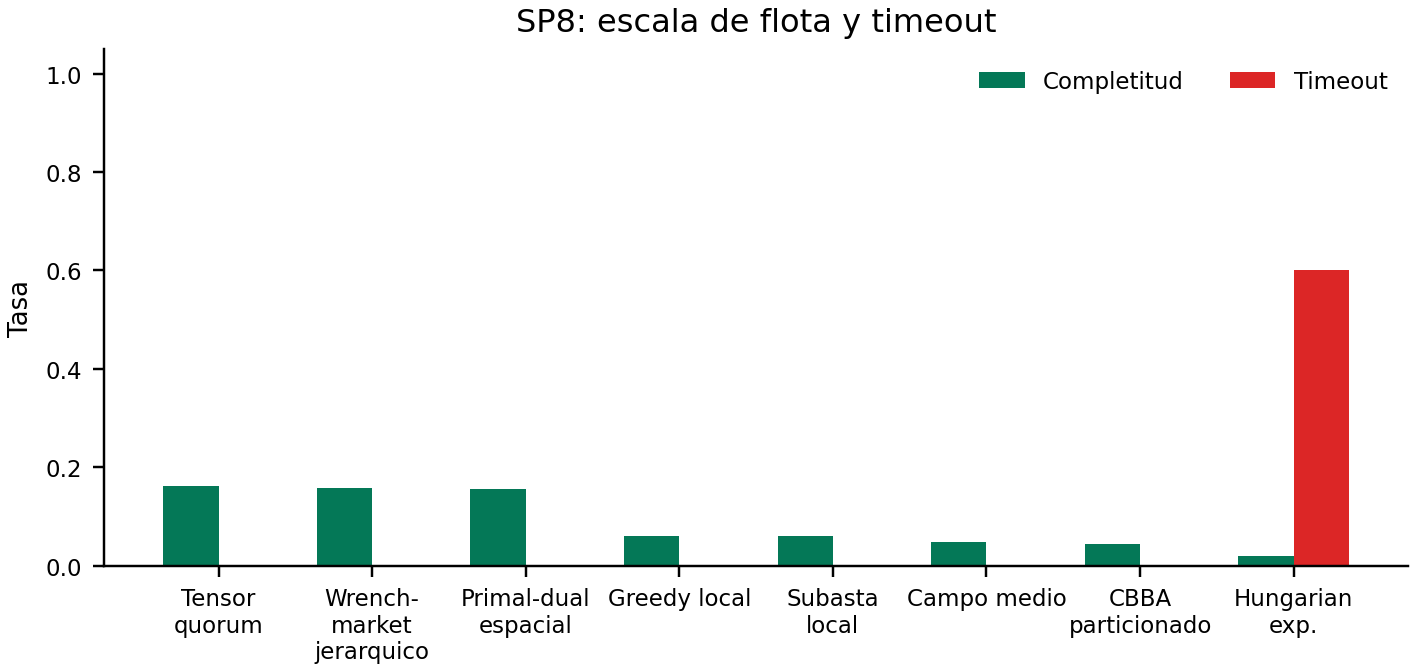
\includegraphics[width=\linewidth]{figures/fig-sp8-primary.png}
\end{minipage}\hfill
\begin{minipage}[t]{0.49\textwidth}
\centering
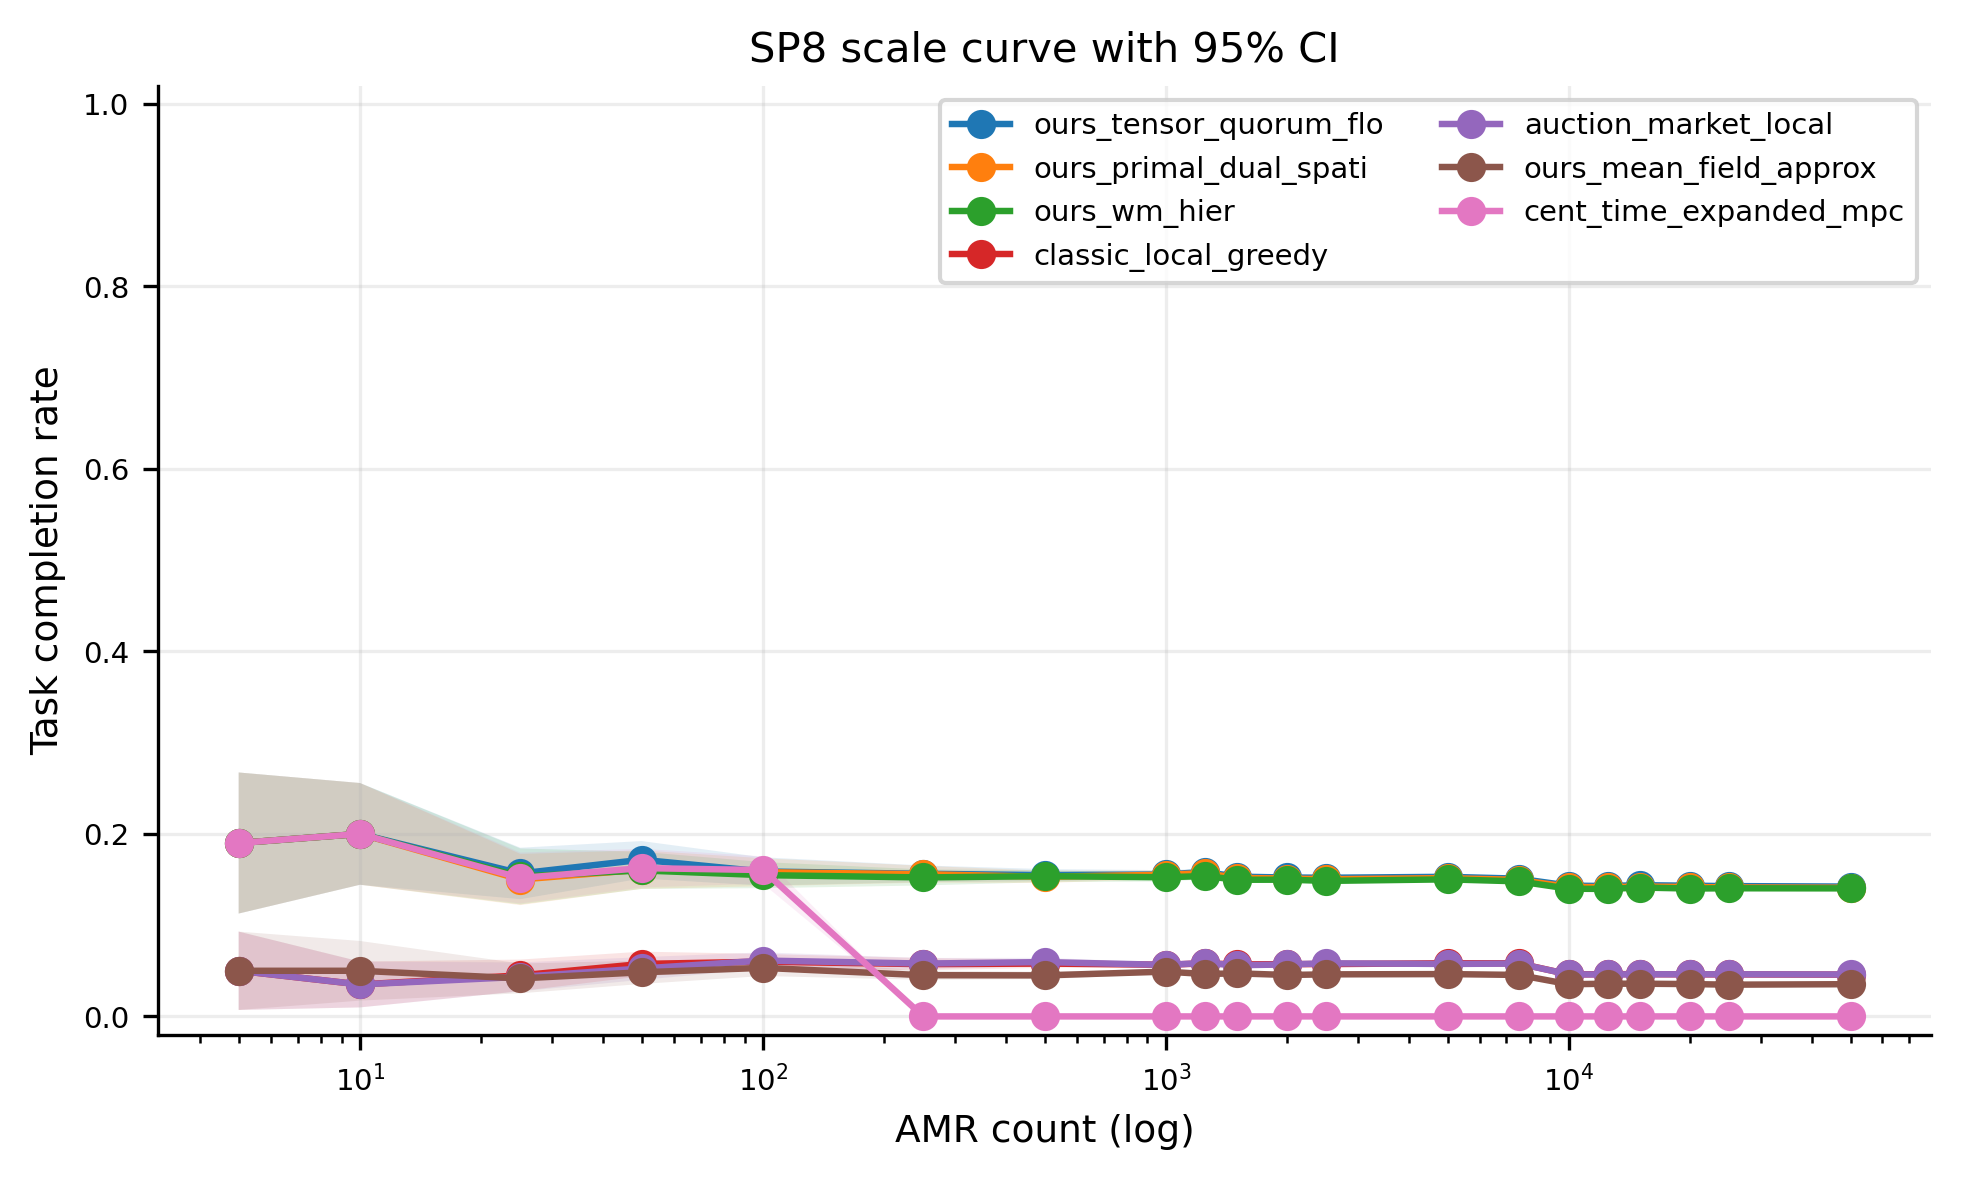
\includegraphics[width=\linewidth]{figures/fig-sp8-scale-ci.png}
\end{minipage}
\caption[Resultados exploratorios de SP8]{Completitud y tendencia con el tamaño en el modelo mesoscópico. Los paneles no validan tiempo o memoria observados.}
\viuownsource
\label{fig:sp8-primary}
\label{fig:sp8-scale-ci}
\end{figure}

En las salidas conservadas, el flujo tensorial registra $0{,}1561$ de completitud y $0{,}1940$ de factibilidad \emph{wrench}; primal-dual obtiene $0{,}1542$ y $0{,}1940$; el mercado jerárquico, $0{,}1529$ y $0{,}1933$; y \emph{greedy} local, $0{,}0521$ de completitud. La diferencia descriptiva entre el mercado jerárquico y \emph{greedy} es $0{,}1008$. Estas magnitudes pertenecen al generador mesoscópico y pueden estar afectadas por funciones de evaluación específicas de cada método.

Los valores históricos de $0{,}6$ y $0{,}8$ asignados al límite del húngaro y del oráculo no proceden de un timeout externo común. Del mismo modo, $2{,}08$ MB, $1254$ MB y $20\,514$ MB son estimaciones analíticas, no RSS observado. No se usan para afirmar que una familia agota antes tiempo o memoria.

\subsubsection{Decisión inferencial}

Las afirmaciones de escalado de recursos basadas en timeout declarado y memoria analítica quedan suspendidas. Los contrastes de calidad almacenados (H8.2--H8.3) se consideran exploratorios pese a sus valores $p$. Una nueva campaña debería ejecutar cada método bajo el mismo timeout externo, medir wall-clock y RSS, conservar la censura y hacer ciego el evaluador a la identidad del método. Hasta entonces, SP8 no demuestra escalabilidad industrial ni superioridad computacional; delimita preguntas y artefactos necesarios para evaluarlas.
